\begin{figure*}
\centering
\includegraphics[width=\textwidth]{res_flux_FHR}
\caption{\label{fig:res-flux-FHR}Relative flux enhancements of $E$ (left column), $L_z$ (middle) and $Q$ (right) for resonance ratios corresponding to the 1:3, 1:2, 2:3 and 3:4 resonances. We show results as computed here with a solid red line, and results from Flanagan, Hughes and Ruangeri (FHR14)~\cite{Flanagan2012a} with a dashed blue line. Each row has a different eccentricity and inclination corresponding to tables I--IV in FHR14. All systems have $a_\ast=0.9$.}
\end{figure*}


The plus-polarisation of the GW at the start and end of the evolution is shown in the top row of \figref{good-waveform}.
\begin{figure*}
\centering
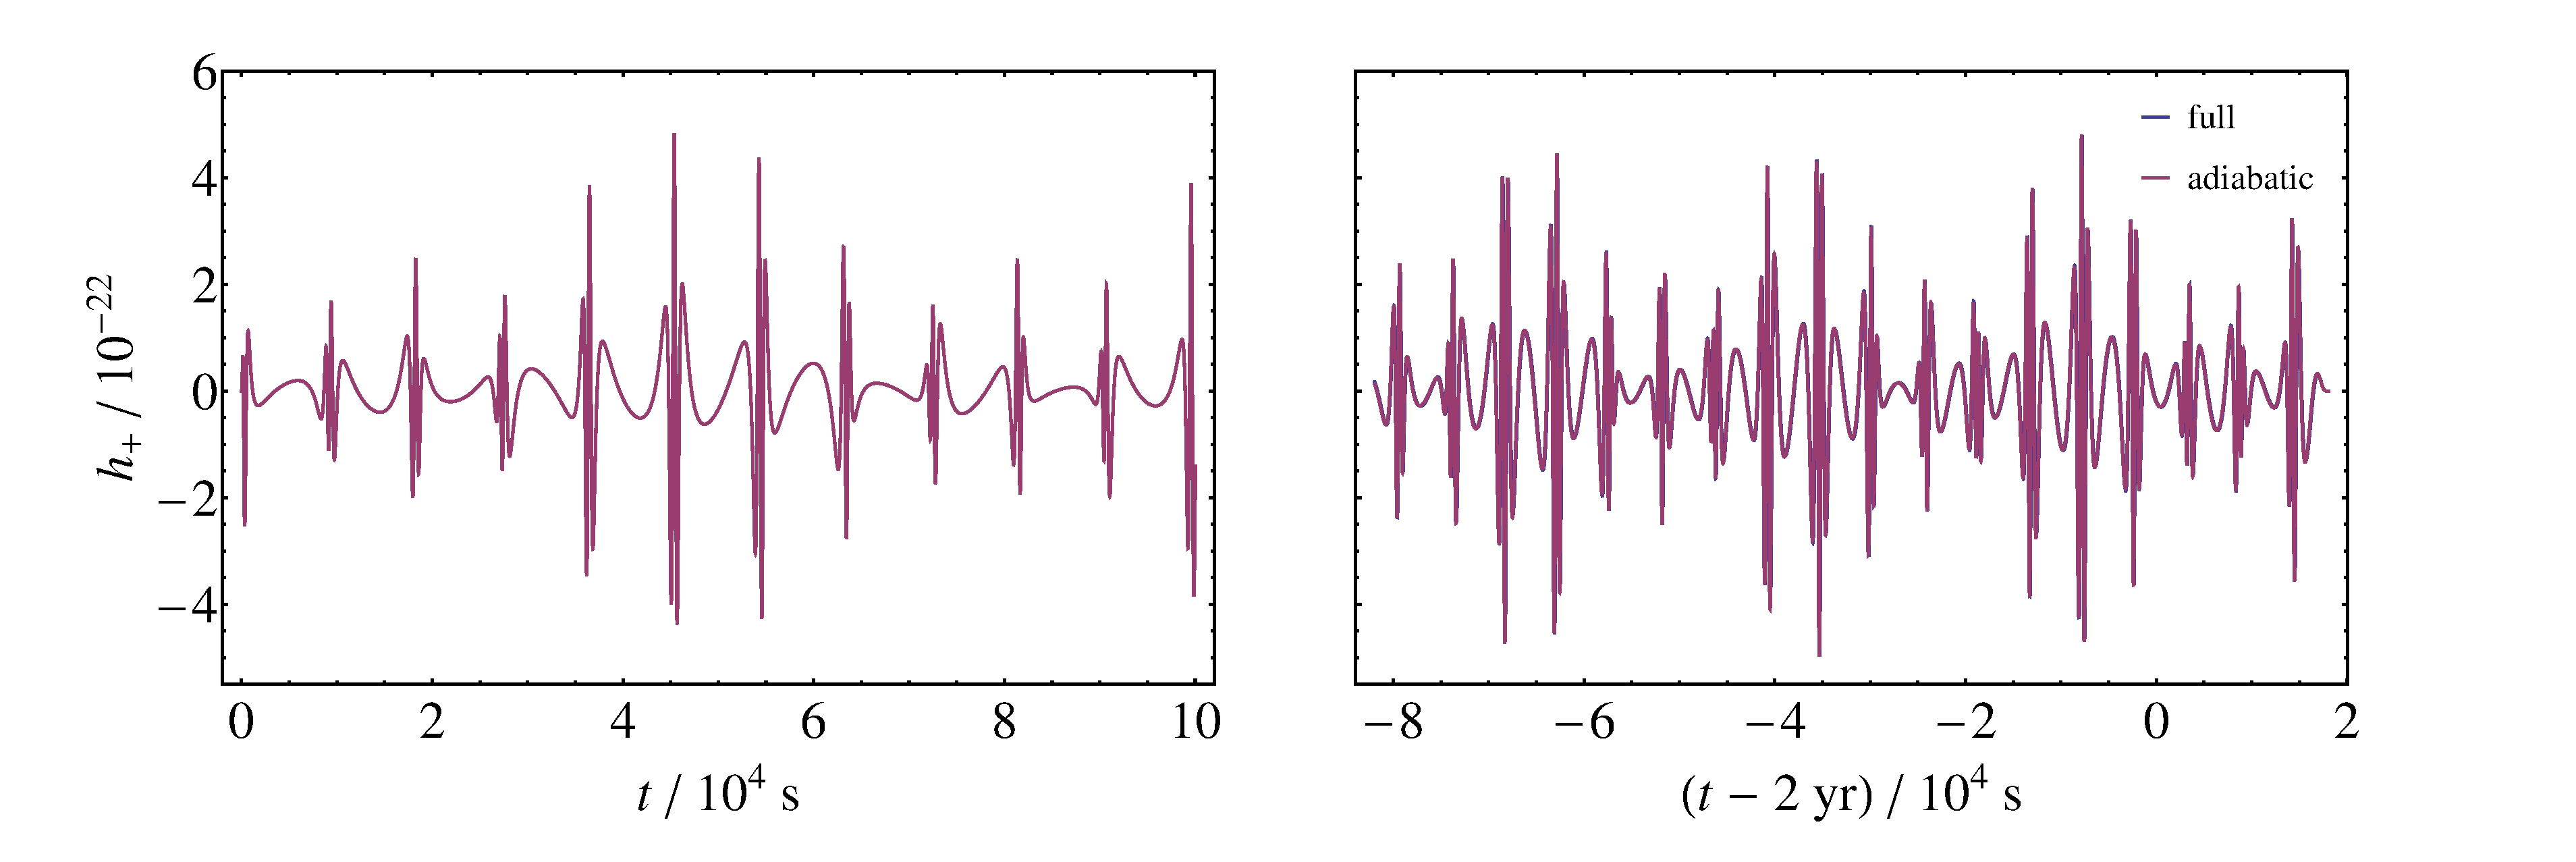
\includegraphics[width=0.92\textwidth]{Fig_good_waveform}
\caption{\label{fig:good-waveform}The plus-polarised waveform for an illustrative EMRI system with initial semi-latus rectum $p_0=7.5$, shown for two short segments at the start and end of a $2$ year evolution. The full and adiabatic models are both shown, but are indistinguishable by eye.}
\end{figure*}

Plotting the plus-polarised GWs at the start and end of the evolution, as before, demonstrates this dephasing, as shown in \figref{dephased-waveform}.
\begin{figure*}
\centering
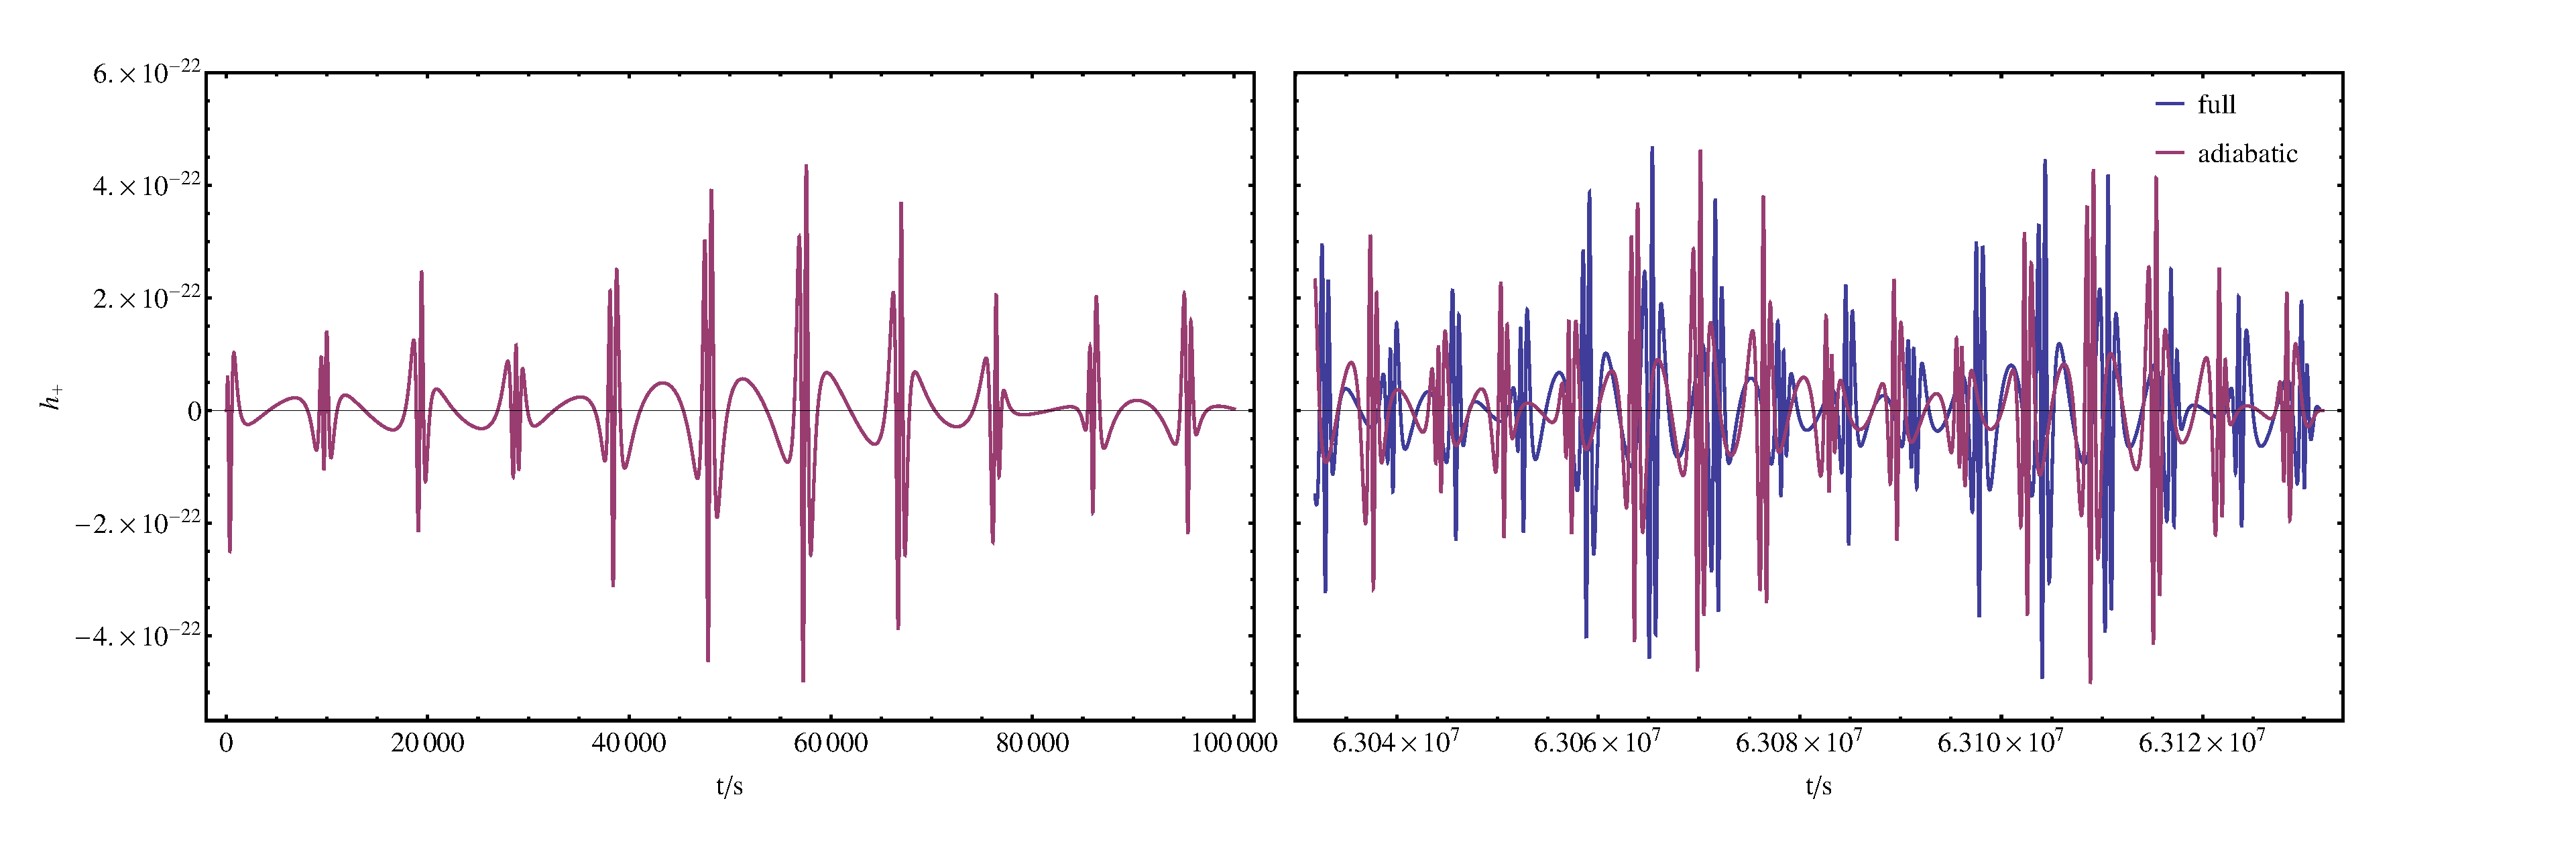
\includegraphics[width=0.92\textwidth]{Fig_dephased_waveform}
\caption{\label{fig:dephased-waveform}The plus-polarised waveform for an illustrative EMRI system with $p=7.85$, shown for two short segments at the start and end of a $2$ year evolution. The full and adiabatic models are both shown; there is a significant dephasing between them by the end of the evolution.}
\end{figure*}


For each system, we compute the overlap between the full evolution and the family of adiabatics given by our set of match times $t\sub{match}$ described in the previous section. The largest overlap in each case, plotted in \figref{overlap-vs-q}, appears to be roughly independent of the value of $q$ and hence with the relative sizes of the orbital parameter jumps.
\begin{figure}
\centering
\includegraphics[width=0.46\textwidth]{overlap_vs_q}
\caption{\label{fig:overlap-vs-q}The overlap between the full and adiabatic evolutions, maximised over the family of generated adiabatics, as a function of the extracted phase parameter $q$. Each dot represents a system with our illustrative parameters and a random choice of the initial radial phase. The red line indicates the expected overlap assuming that the waveforms match exactly post-resonance, but have zero overlap pre-resonance.}
\end{figure}
The best performing adiabatic for the majority of our systems matched at the end of the inspiral. We can therefore estimate the value of the overlap by assuming that the adiabatic waveforms recover the entire SNR in the region post-resonance, but none at all in the region pre-resonance. We expect the overlap to scale with the fraction of time spent post-resonance, the value of which is demonstrated by the red line in \figref{overlap-vs-q}. There is not an exact equivalence because of the frequency-dependent noise of eLISA; cycles near the end of the inspiral accumulate proportionally more SNR at a frequency closer to the minimum of the eLISA noise curve.
Systems with $|q| \approx \pi/2$ (corresponding to small jumps in $E$ and $L_z$) have higher than average overlaps due to additional accumulation in the pre-resonance region. The adiabatic models of these systems dephase more slowly, but still do not produce very high overlaps due to the jump in $Q$. A small fraction of systems have a lower overlap than expected, at around $0.5$. This is due to a sub-optimal choice of the matching times; making small adjustments to $t\sub{match}$ can lead to higher overlaps, but the exact adjustments required are difficult to predict in advance.


After computing the SNRs of our NK waveforms for each of the $513$ EMRI systems, we can compare the values to those obtained using the AK formalism. The different approximation schemes are expected to produce different results, but they should be broadly similar. In \figref{pop-SNR-vs-eta}, we plot the ratio of the new NK SNR to the AK SNR, as a function of the mass ratio. We observe a clear trend, with systems closest to equal mass performing roughly as expected, but with the most extreme systems giving significantly lower SNRs. This is a consequence of the PN self-force model we are using, which we have found overestimates the inspiral rate for EMRIs. Detectable systems with larger mass ratios (closer to equal mass) plunge at higher frequencies, and so during the $2\units{yr}$ observation window, they evolve within the bucket of the eLISA noise curve. Increasing the rate of evolution then does not significantly change the recovered SNR since we are still sensitive to all parts of the waveform. At smaller mass ratios, the systems evolve more slowly, from lower plunge frequencies. An increased evolution rate means that earlier portions of the EMRI are shifted outside the sensitive region of the detector, thus giving a much lower SNR.
\begin{figure}
\centering
\includegraphics[width=0.46\textwidth]{pop_SNR_vs_eta}
\caption{\label{fig:pop-SNR-vs-eta}The ratio of SNRs as computed with waveforms generated using the NK (adopting our PN self-force model) and AK formalisms, as a function of (the base-10 logarithm of) the mass ratio. Each system has an AK SNR greater than $15$, using the eLISA detector with 6 laser links.}
\end{figure}
We can study the effect of resonances, by comparing the maximum adiabatic SNR to the full SNR computed using the NK waveforms. The resulting overlap is still indicative of the effect of resonances on the population of systems.
%\begin{figure}
%\centering
%\includegraphics[width=0.46\textwidth]{pop_adSNR_vs_Tad}
%\caption{\label{fig:pop-adSNR-vs-Tad}The maximum overlap for $513$ detectable EMRI systems obtained by comparing the instantaneous evolution with each of the adiabatic models in our one-parameter family. Each system encounters either $0$ (blue squares), $1$ (gold triangles) or $2$ (green circles) resonances during the observation window $t\sub{insp}$. The overlap is plotted against the largest time spent by the inspiral without encountering any resonances $t\sub{ad}$, normalised by $t\sub{insp}$. The solid line corresponds to the expected value if the $1$:$2$ and $2$:$3$ resonances cause significant waveform dephasing.}
%\end{figure}
